\documentclass[11pt]{article}
\usepackage[utf8]{inputenc}
\usepackage[T1]{fontenc}
\usepackage{amsmath,amssymb,amsthm}
\newtheorem{assumption}{Assumption}
\newtheorem{lemma}{Lemma}
\newtheorem{theorem}{Theorem}
\newtheorem{proposition}{Proposition}
\newtheorem{corollary}{Corollary}
\newtheorem{remark}{Remark}
\usepackage{graphicx}
\usepackage{booktabs}
\usepackage[margin=1in]{geometry}
\usepackage[round]{natbib}
\usepackage{caption}
\usepackage{hyperref}

% Figure search paths: the first three work from companion_papers/CCR_measurement_paper/
% in the project folder; the last three work from paper/ in the public repository.
\graphicspath{{../../experiments/empirical/figures/}{../../experiments/empirical/ablation/figures/}{../../experiments/figures/}{../experiments/empirical/figures/}{../experiments/empirical/ablation/figures/}{../experiments/figures/}}
\bibliographystyle{apalike}

%% NOTE (for CCR submission): initial submission may be APA7 (this file) or the
%% CCR LaTeX template; the CCR template is required only on acceptance. This file
%% is the NAMED working master; produce an anonymized copy for review (strip
%% authors/affiliations, replace the companion self-citation with "(Author, 2026)",
%% and remove the GitHub/Zenodo links).

\title{Measuring Aesthetic Homogenization in Text-to-Image AI:\\ Diversity Collapse in DALL-E 3 and Imagen 4}

\author{%
Timothy Graham,$^{1,*}$ Sadia Sharmin,$^{1}$ Daniel Whelan-Shamy,$^{1}$ Vish Padinjaredath Suresh,$^{1}$\\
Rayane El Masri,$^{1}$ Amelia Radke,$^{2}$ Aaron Snoswell,$^{1}$ Jean Burgess,$^{1}$ Daniel Angus,$^{1}$\\
Kevin Witzenberger,$^{1}$ Samantha Vilkins,$^{1}$ Sebastian Svegaard,$^{1}$ Shaghayegh Mohammadamini,$^{1}$\\
Will He,$^{1}$ Guangnan Zhu,$^{1}$ Abdul Obeid,$^{1}$ Kunal Chand,$^{1}$ Anand Badola,$^{1}$ Khanh Luong,$^{1}$\\
Caroline Gardam,$^{1}$ Ashwin Nagappa$^{1}$\\[6pt]
\small $^{1}$Digital Media Research Centre, Queensland University of Technology, Brisbane, Australia\\
\small $^{2}$Independent Researcher, Brisbane, Australia\\
\small $^{*}$Corresponding author: Timothy.Graham@qut.edu.au}
\date{}

\begin{document}
\maketitle

\begin{abstract}
Text-to-image models produce outputs that are strikingly similar to one another, but the scale of this homogenization has not been systematically measured. We introduce a reproducible methodology for quantifying aesthetic and cultural diversity collapse in generative image models, operationalizing three distributional measures - effective support radius, diversity index, and effective dimension - in CLIP and DINOv2 embedding space. Applying the method to 1,177 images from two leading commercial models, DALL-E 3 and Imagen 4, we find that within-prompt outputs collapse to about 10 of 768 effective dimensions, discarding over 98\% of available variation; that minority cultural representations are 17\% less diverse than majority ones ($p < 0.001$, Hedges' $g = 1.51$); and that the two independently developed models converge to cosine similarity 0.86 on identical prompts, well above the 0.64 baseline that mismatched prompts produce. A controlled ablation on open-source models (Stable Diffusion XL) isolates the mean-squared-error objective from preference training and shows that, at the standard guidance scale, 91\% of the majority/minority diversity gap is already present in a base model with no preference training, while classifier-free guidance monotonically compresses diversity. The homogenization is therefore primarily structural - a property of the objective rather than of human-feedback tuning. We release all code and embeddings; the cultural interpretation is developed in a companion paper.
\end{abstract}

\noindent\textbf{Keywords:} text-to-image generation, diffusion models, aesthetic diversity, cultural representation, CLIP embeddings, computational methods

\section{Introduction}

Diffusion-based text-to-image models such as DALL-E \citep{Ramesh2021}, Stable Diffusion \citep{Rombach2022}, and Imagen have moved quickly from research artifacts to infrastructure for the production of visual culture. A persistent observation accompanies their adoption: their outputs tend to look alike, converging on a generic ``AI aesthetic'' of smooth surfaces, conventional composition, and culturally flattened representation. This observation is now widespread in qualitative and critical scholarship, but it has rarely been \emph{measured}. How much diversity do these systems actually discard? Do they compress the representation of some cultures more than others? And do independently developed models converge on the same visual center? These are empirical, quantifiable questions, and answering them is a prerequisite for any claim - technical, cultural, or regulatory - about homogenization.

This paper contributes a reproducible computational methodology for measuring aesthetic and cultural diversity collapse in text-to-image models, and applies it to two leading commercial systems and a controlled open-source ablation. Our approach operationalizes diversity as the geometry of a model's outputs in a semantic embedding space: for a fixed prompt, we generate many independent images, embed them, and quantify how tightly the resulting cluster is concentrated using three complementary distributional measures. Low diversity means the model returns nearly the same image every time; systematically lower diversity for some prompts than others reveals \emph{whose} representations are compressed hardest.

We report three findings. First, within-prompt outputs from DALL-E 3 and Imagen 4 occupy only about 10 effective dimensions out of 768, discarding over 98\% of the available variation. Second, prompts naming minority nationalities yield 17\% less within-prompt diversity than majority ones ($p < 0.001$), an empirical signature of stronger homogenization for less-represented cultures. Third, DALL-E 3 and Imagen 4 - built by different companies on different data - converge to cosine similarity 0.86 across identical prompts, where mismatched prompts across the same two models average only 0.64. A controlled ablation on Stable Diffusion XL then isolates the cause: at the standard guidance scale, 91\% of the majority/minority diversity gap is already present in a base model trained only with the mean-squared-error (MSE) denoising objective, before any preference training, and classifier-free guidance compresses diversity further and monotonically.

We give a formal account of the mechanism behind these measurements - why the MSE denoising objective structurally averages aesthetic modes in proportion to their statistical mass, and how classifier-free guidance amplifies the effect - in Section~\ref{sec:mechanism}, and validate it on synthetic data before measuring it in real systems. The broader cultural and critical interpretation of the findings - what a statistical monoculture means for visual culture, representation, and governance - is developed in a companion paper \citep{Companion2026}.

In summary, this paper makes four contributions. (1) A formal account of the mechanism: we show that the MSE denoising objective computes a mode-averaging conditional expectation, that classifier-free guidance amplifies it, and that both reduce three distributional measures of diversity. (2) A reproducible, model-agnostic \emph{methodology} for measuring aesthetic and cultural diversity collapse in text-to-image models, validated on synthetic data with known ground truth. (3) An \emph{empirical characterization} of homogenization in two leading commercial systems - within-prompt concentration, minority-culture suppression, and cross-model convergence - replicated across two embedding models. (4) A controlled \emph{ablation} on open-source models that attributes the majority of the effect to the training objective rather than to preference training. All prompts, generation and analysis code, and precomputed embeddings are released.

\section{Related work}\label{sec:related}

Our study connects three strands of research: bias and representation in text-to-image models, the measurement of generative diversity, and model collapse.

\paragraph{Bias and cultural representation.} A substantial literature documents demographic and cultural bias in text-to-image outputs. \citet{Bianchi2023} show that simple, everyday prompts amplify demographic stereotypes at scale; \citet{Luccioni2023} evaluate societal representations across occupations; and \citet{Ghosh2023} find that under-specified prompts such as ``a person'' default to light-skinned Western men. \citet{Seshadri2023} examine the relationship between training-data skew and output bias, and cross-cultural benchmarks such as CultDiff \citep{Bayramli2025} show that state-of-the-art models fail to render culturally accurate artifacts for underrepresented regions. \citet{AlDahoul2025} document racial homogenization in generated faces, and \citet{Kotliar2020} theorizes the algorithmic construction of a non-Western ``other.'' This work establishes \emph{that} outputs are biased and catalogs specific stereotypes. Our contribution is complementary and methodological: a general procedure for quantifying \emph{how much} within-category diversity is lost, and for whom, that applies uniformly across models and prompt types rather than enumerating particular failures.

\paragraph{Measuring generative diversity.} Standard generative-model metrics such as the Fr\'echet Inception Distance summarize the distance between generated and reference distributions but do not isolate \emph{within-prompt} diversity or attribute concentration to particular conditioning. We instead compute per-prompt distributional measures - spread, entropy, and effective dimension - directly in embedding space, drawing on the participation ratio from statistical physics and differential entropy from information theory \citep{Shannon1948}. This makes diversity a per-prompt, per-group quantity that can be compared across cultures, categories, and models, and that connects directly to the conditional-expectation mechanism.

\paragraph{Model collapse and diversity-preserving generation.} Recursive training on model-generated data degrades diversity across successive model generations \citep{Shumailov2024, Alemohammad2023, Shumailov2023}, an effect \citet{Schaeffer2025} qualify with respect to data accumulation. Our cross-model convergence result is a static, single-generation analogue: independently trained models already occupy nearly the same aesthetic center, and recursive contamination would compound this over time. On the mitigation side, methods such as Fair Diffusion \citep{Friedrich2023} and quality-diversity sampling \citep{Chang2024} intervene to broaden outputs; the measurements we propose provide an evaluation target against which such interventions can be assessed.

\section{Measuring aesthetic diversity}\label{sec:metrics}

\subsection{Distributional measures}

We treat a semantic embedding space $\mathcal{X}$ as the operationalization of ``aesthetic space,'' in which images with similar content and style map to nearby points. For a set of images generated from one prompt, embedded as vectors in $\mathcal{X}$, we compute three measures of concentration:

\begin{itemize}
 \item \textbf{Effective support radius} $R_\alpha$: the $\alpha$-percentile distance of the embeddings from their centroid ($\alpha = 90$), measuring the spatial spread of the output cluster.
 \item \textbf{Diversity index} $D$: a per-dimension normalized Gaussian-fit entropy, $\exp(H/k)$, computed from the $k$ non-degenerate eigenvalues of the sample covariance (with $n$ samples in $d \gg n$ dimensions the covariance has rank at most $n-1$).
 \item \textbf{Effective dimension} $d_{\mathrm{eff}}$: the participation ratio of the eigenvalue spectrum of the sample covariance, $d_{\mathrm{eff}} = (\sum_i \lambda_i)^2 / \sum_i \lambda_i^2$, measuring how many independent directions of variation the outputs span.
\end{itemize}

Low values on all three indicate that a model's outputs for a prompt are concentrated near a single point - the behavior predicted when the model returns an approximate conditional expectation. To compare an output distribution $Q$ against a reference $P$ we use the corresponding ratios $\rho_\alpha = R_\alpha(Q)/R_\alpha(P)$, $\delta = D(Q)/D(P)$, and $\gamma = d_{\mathrm{eff}}(Q)/d_{\mathrm{eff}}(P)$; values below 1 indicate homogenization. These measures are standard in information theory and statistical physics (the participation ratio) and are well defined in the high-dimensional spaces in which generative models operate.

\subsection{Embedding spaces}

We embed images with CLIP ViT-L/14 \citep{Radford2021}, producing $\ell_2$-normalized 768-dimensional vectors, and replicate the central analyses with DINOv2 \citep{Oquab2024}, a self-supervised encoder trained without language supervision, to confirm that the findings are not an artifact of CLIP's text-image training. Agreement across the two encoders indicates that the measured concentration reflects the images themselves rather than any single representation.

\subsection{Computation and reproducibility}

The three measures are computed from the sample covariance of a prompt's embeddings. The effective support radius is the 90th percentile of Euclidean distances from the centroid; the diversity index uses a Gaussian-fit differential entropy evaluated on the non-degenerate covariance spectrum - the top $\min(n-1, d)$ eigenvalues above a relative floor, normalized per retained dimension, a restriction that makes the estimator deterministic across linear-algebra implementations; and the effective dimension is the participation ratio of the covariance eigenvalues. Because these are second-order statistics of a modest number of samples per prompt (typically 20), we quantify their sampling variability with a nonparametric bootstrap (10,000 resamples per prompt) and assess group differences with a permutation test (10,000 permutations), reporting both confidence intervals and $p$-values. The full pipeline - prompt set, generation scripts, embedding extraction, and metric computation - is released, and the analysis can be reproduced directly from the published embeddings without regenerating images, so results do not depend on continued API access to the commercial models.

\section{The mode averaging mechanism}\label{sec:mechanism}

We now show why these measures should be small for diffusion models: the training objective is, by construction, an averaging operator. This section states the mechanism formally; it motivates and predicts the measurements that follow.

\subsection{The objective is a conditional expectation}

A diffusion model \citep{Ho2020, Song2021} adds Gaussian noise to data $x_0$ over $T$ steps, $x_t = \sqrt{\bar{\alpha}_t}\,x_0 + \sqrt{1-\bar{\alpha}_t}\,\epsilon$ with $\epsilon \sim \mathcal{N}(0,I)$ and noise variance $\sigma_t^2 = 1-\bar{\alpha}_t$, and trains a network $\epsilon_\theta(x_t,t)$ to predict the noise by minimizing the mean-squared error $\mathbb{E}[\|\epsilon - \epsilon_\theta(x_t,t)\|^2]$. The minimizer of this loss is the conditional expectation $\mathbb{E}[\epsilon \mid x_t]$, equivalently (by reparameterization) $\mathbb{E}[x_0 \mid x_t]$: the model learns the \emph{average} of all clean images consistent with the noised input. That the optimal denoiser is a conditional expectation is standard \citep{Ho2020}; our concern is its consequence for diversity, because a conditional expectation neither selects the most likely mode nor preserves rare ones - it returns a weighted mean.

\subsection{A mixture model of aesthetic data}

\begin{assumption}[Mixture of aesthetic modes]\label{assum:mixture}
The data distribution is a mixture $P_{\mathrm{data}}(x) = \sum_{i=1}^k \pi_i\,\mathcal{N}(x;\mu_i,\Sigma_i)$, with mixing weights $\pi_i>0$ ($\sum_i \pi_i = 1$) giving the \emph{statistical mass} of each aesthetic mode, means $\mu_i$ its center, covariances $\Sigma_i$ its internal diversity, and well-separated components ($\|\mu_i-\mu_j\|\ge\delta>0$).
\end{assumption}

Real aesthetic data clusters into identifiable styles with very unequal prevalence in web-scraped corpora; the weights $\pi_i$ encode this asymmetry, with dominant modes (e.g., Western stock photography) carrying large mass and minority modes small mass.

\subsection{Mode averaging under high noise}

\begin{lemma}[Within-mode shrinkage]\label{lem:shrinkage}
Under the diffusion process, for a Gaussian mode $C_i$,
$\mathbb{E}[x_0 \mid x_t, C_i] = \mu_i + \bar{\alpha}_t\Sigma_i(\bar{\alpha}_t\Sigma_i + \sigma_t^2 I)^{-1}\!\left(\tfrac{x_t}{\sqrt{\bar{\alpha}_t}} - \mu_i\right)$,
and in the terminal-noise limit $t \to T$, where the signal-to-noise ratio $\mathrm{SNR}_t = \bar{\alpha}_t/\sigma_t^2 \to 0$, the shrinkage factor vanishes, so $\mathbb{E}[x_0 \mid x_t, C_i] \to \mu_i$.
\end{lemma}

The lemma follows from the standard Gaussian conditioning formula applied to the joint law of $(x_0,x_t)$ given $C_i$; at terminal noise the observation carries vanishing information about position within a mode, and the estimate collapses to the mode center. (In the variance-preserving parameterization $\sigma_t^2 = 1-\bar{\alpha}_t \le 1$, so the relevant limit is $\bar{\alpha}_t \to 0$ rather than $\sigma_t \to \infty$; all statements below are taken in this low-SNR limit.)

\begin{theorem}[Mode Averaging Principle]\label{thm:MAP}
Under Assumption~\ref{assum:mixture}, as $\mathrm{SNR}_t \to 0$ the optimal denoiser satisfies:
(1) \textbf{Mode averaging:} $\mathbb{E}[x_0 \mid x_t] = \sum_i P(C_i \mid x_t)\,\mathbb{E}[x_0 \mid x_t, C_i] \to \sum_i \pi_i\mu_i = \mu_{\mathrm{global}}$; and
(2) \textbf{Prior transmission:} the posterior over modes converges to the prior, $P(C_i \mid x_t) \to \pi_i$.
\end{theorem}

\begin{proof}[Proof sketch]
By the law of total expectation and Lemma~\ref{lem:shrinkage}, the within-mode terms tend to $\mu_i$. For the posterior, Bayes' rule gives $P(C_i\mid x_t) \propto \pi_i\,\mathcal{N}(x_t;\sqrt{\bar{\alpha}_t}\mu_i, \bar{\alpha}_t\Sigma_i+\sigma_t^2 I)$. When $\sigma_t^2 \gg \bar{\alpha}_t\|\Sigma_i\|$, every component covariance is $\approx \sigma_t^2 I$; the determinant prefactors equalize and the $\mu_i$-dependent terms in the exponent are $O(\bar{\alpha}_t/\sigma_t^2)\to 0$, so the likelihoods equalize and $P(C_i\mid x_t)\to\pi_i$. Substituting yields $\mathbb{E}[x_0\mid x_t]\to\sum_i\pi_i\mu_i$.
\end{proof}

By standard universal-approximation arguments, a sufficiently expressive network trained to the MSE optimum inherits this behavior, so the effect applies to any diffusion model trained with the MSE objective - including all major text-to-image systems. Prior transmission is the key point for diversity: a mode with mass $\pi_i = 0.03$ contributes only 3\% to the output regardless of the input, so the training data's cultural asymmetry is structurally preserved, and minority modes are pulled toward the dominant center.

\subsection{Classifier-free guidance amplifies concentration}

Classifier-free guidance (CFG) replaces the noise prediction with $\tilde{\epsilon}_\theta = (1+w)\epsilon_\theta(x_t,c,t) - w\,\epsilon_\theta(x_t,t)$ for a guidance scale $w>0$ \citep{Ho2022, Dhariwal2021}, the standard technique for improving prompt fidelity and perceived quality.

\begin{proposition}[CFG sharpens the conditional]\label{prop:cfg}
The CFG update follows the score of $\tilde{p}(x_t\mid c) \propto p(x_t\mid c)^{1+w} / p(x_t)^{w}$. For $w>0$ this raises the conditional density to a power greater than one, sharpening its peaks and attenuating its tails. Provided the conditional is no more diffuse than the marginal - for Gaussian approximations $p(x_t \mid c) \approx \mathcal{N}(\mu_c, \Sigma_c)$ and $p(x_t) \approx \mathcal{N}(\mu_0, \Sigma_0)$ with $\Sigma_c \preceq \Sigma_0$, the generic situation since conditioning narrows the distribution - the effective sampling distribution has smaller covariance than under standard conditional generation.
\end{proposition}

\begin{proof}
Writing $\tilde{s} = \nabla_{x_t}[(1+w)\log p(x_t\mid c) - w\log p(x_t)]$ identifies the target density as $p(x_t\mid c)^{1+w}/p(x_t)^{w}$. For the Gaussian approximations, completing the square gives a Gaussian with precision $(1+w)\Sigma_c^{-1} - w\Sigma_0^{-1} = \Sigma_c^{-1} + w(\Sigma_c^{-1} - \Sigma_0^{-1}) \succeq \Sigma_c^{-1}$ whenever $\Sigma_c \preceq \Sigma_0$, so the effective covariance satisfies $[(1+w)\Sigma_c^{-1} - w\Sigma_0^{-1}]^{-1} \preceq \Sigma_c$, with equality only when $\Sigma_c = \Sigma_0$ (in which case guidance shifts the mean without changing the covariance).
\end{proof}

Because the conditional is already a prior-weighted average (Theorem~\ref{thm:MAP}), CFG narrows an already-concentrated prediction: the mechanism used to make images look ``better'' simultaneously makes them more generic. In deterministic (DDIM) sampling the high-noise average also fixes which mode a trajectory falls into, so per-step averaging carries through to the final output; commercial systems typically use large $w$ ($\ge 7$), making this lock-in strong in practice. Two caveats bound the scope of the formal argument. First, the guided update follows the score of $\tilde{p}$ at each noise level but does not exactly sample $\tilde{p}$ over a full trajectory. Second, an exact score model with fully stochastic ancestral sampling would in principle reproduce its training distribution; the collapse operates through the interaction of the averaged prediction with guidance, deterministic or few-step samplers, and imperfect score estimation. This is why we treat the mechanism as generating testable predictions and verify them empirically (Sections~\ref{sec:synthetic}-\ref{sec:ablation}) rather than relying on the idealized limit.

\subsection{The homogenization corollary}

\begin{corollary}[Homogenization prediction]\label{cor:homogen}
Let $Q$ be the output distribution and $P$ the training distribution. Under Assumption~\ref{assum:mixture}, in the averaging regime of Theorem~\ref{thm:MAP} and with guidance as in Proposition~\ref{prop:cfg}, all three diversity ratios are predicted to fall below one: $\rho_\alpha(Q,P)<1$ (support concentration), $\delta(Q,P)<1$ (diversity loss), and $\gamma(Q,P)<1$ (dimensional collapse).
\end{corollary}

Mode averaging concentrates outputs near dominant mode centers, CFG reduces within-mode variance, and prior transmission drops the effective number of contributing modes; each shrinks the support radius, the entropy, and the participation ratio of $Q$ relative to $P$. These are exactly the quantities the measures of Section~\ref{sec:metrics} estimate, giving four testable predictions: outputs are tightly concentrated for a fixed prompt; concentration is stronger for lower-mass (minority) prompts; CFG monotonically increases it; and independently trained models converge to similar centers. The rest of the paper tests these predictions. Full derivations, together with the cultural and critical reading of the results, are developed in the companion paper \citep{Companion2026}.

\section{Synthetic validation}\label{sec:synthetic}

Before turning to commercial systems, we validate the measures on synthetic data where the ground-truth distribution is known. We construct a three-component Gaussian mixture in $\mathbb{R}^2$ with well-separated modes and asymmetric prior weights ($\pi = 0.70, 0.20, 0.10$), so that the global mean $(2.7, 0.3)$ lies close to the dominant mode. Running the analytic forward-diffusion process and computing the conditional expectation $\mathbb{E}[x_0 \mid x_t]$ across noise levels reproduces every predicted behavior: under high noise the conditional expectation converges to the prior-weighted global mean (mean distance $2.96 \times 10^{-5}$); the posterior over modes converges to the prior (mean absolute deviation $1.22 \times 10^{-6}$), so the data's mass asymmetry is transmitted faithfully; all three homogenization ratios fall below 1; classifier-free guidance decreases them monotonically with guidance scale; and the minority mode's output share falls from its prior of $0.10$ to $0.00$ at high noise. These controlled results confirm that the measures behave as intended and that the averaging mechanism of Section~\ref{sec:mechanism} produces exactly the concentration they detect (Figure~\ref{fig:synthetic}); code is released with this paper.

\begin{figure}[t]
 \centering
 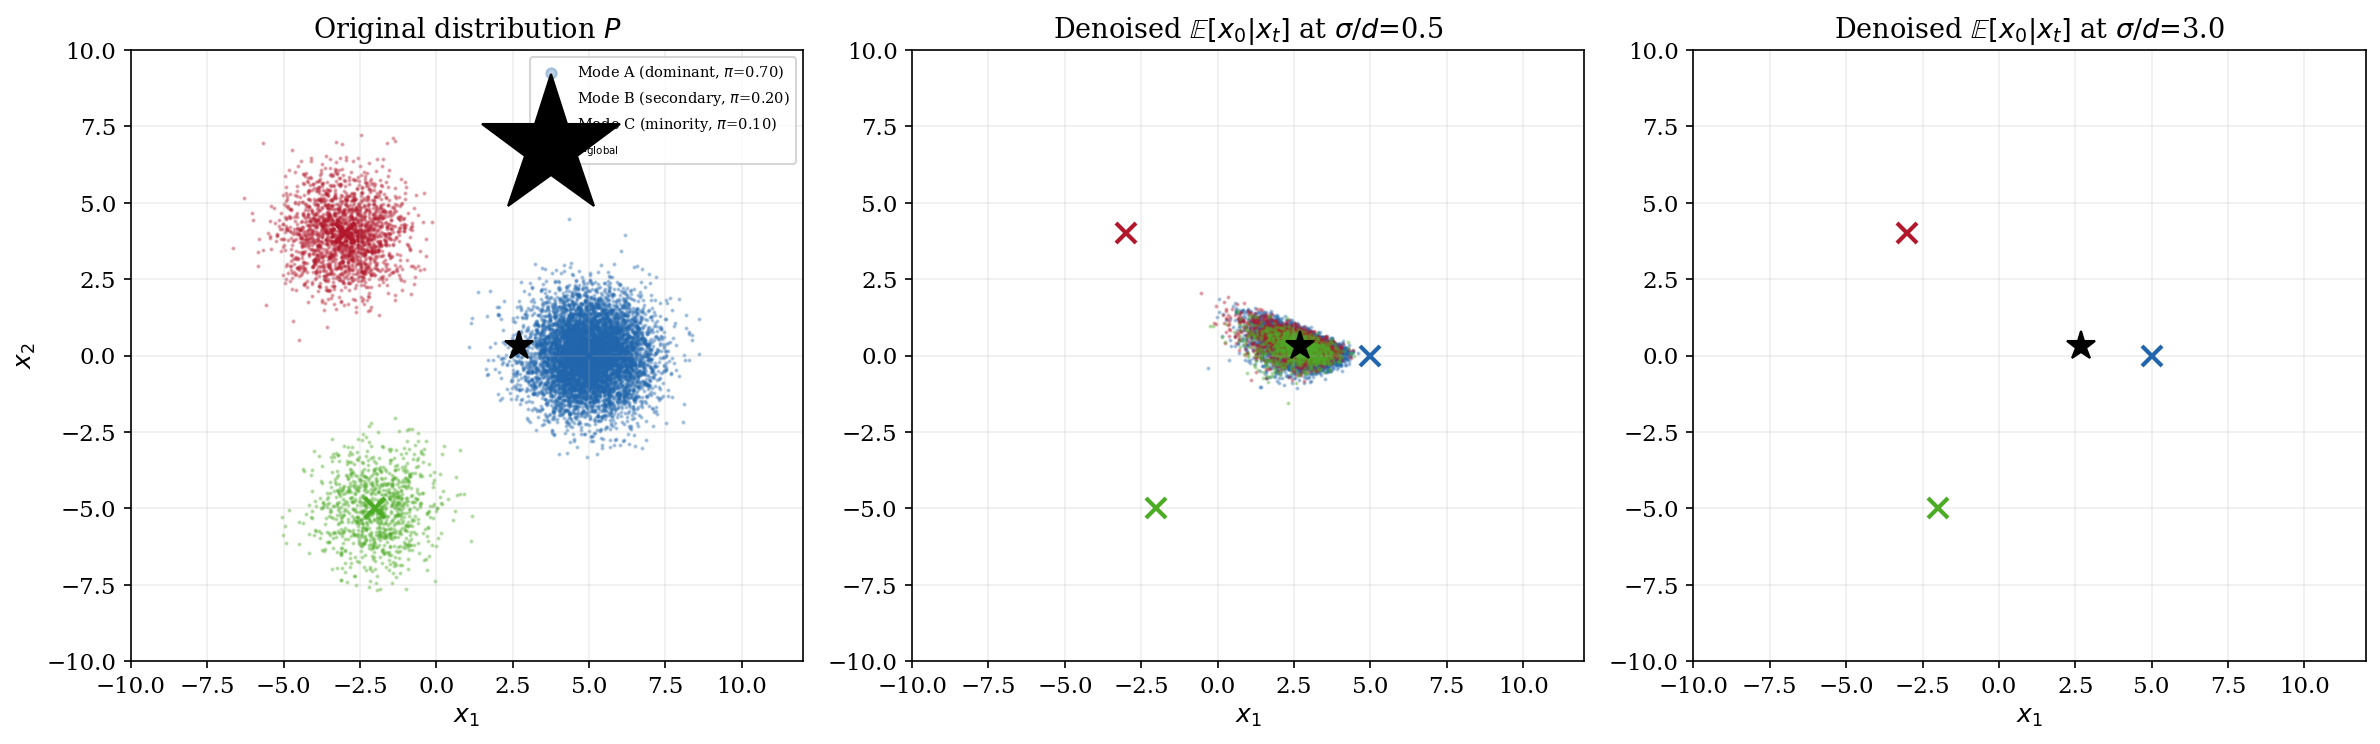
\includegraphics[width=\textwidth]{overview_scatter.png}
 \caption{Synthetic validation on a three-component Gaussian mixture. Left: samples from the training distribution $P$, colored by mode. Center: the conditional expectation $\mathbb{E}[x_0 \mid x_t]$ at moderate noise, already contracting toward the prior-weighted global mean. Right: at high noise the outputs collapse onto the dominant mode, and the minority mode's output share falls to zero - the concentration the three measures are designed to detect.}
 \label{fig:synthetic}
\end{figure}

\section{Empirical study: commercial models}\label{sec:empirical}

\subsection{Design}

We designed 30 prompts in three categories. \emph{Cultural identity} prompts ($n = 15$) take the form ``A photograph of a [nationality] woman,'' with five majority nationalities (American, British, French, Australian, Canadian), selected for high representation in English-language web corpora, and ten minority nationalities (Bangladeshi, Nigerian, Peruvian, Mongolian, Maori, Ethiopian, Uzbek, Guatemalan, Samoan, Kurdish). \emph{Open-ended} prompts ($n = 10$) impose minimal constraints (e.g., ``A beautiful landscape,'' ``An ideal home''), maximizing the model's freedom to default to a dominant aesthetic. \emph{Artistic style} prompts ($n = 5$) request ``A painting of a forest in [style] style'' across two majority styles (Impressionism, Cubism) and three minority styles (Ukiyo-e, Aboriginal dot painting, Persian miniature).

For each prompt we generated 20 independent images from DALL-E 3 (via the OpenAI API, $1024 \times 1024$; 598 images after occasional API errors) and from Imagen 4 (via the Google Gemini API; 579 images after occasional safety filtering), for a combined dataset of 1,177 images. All images were embedded with CLIP ViT-L/14, and the three measures were computed for each prompt's output cluster. Example generations are shown in Figure~\ref{fig:grid}.

\begin{figure}[t]
 \centering
 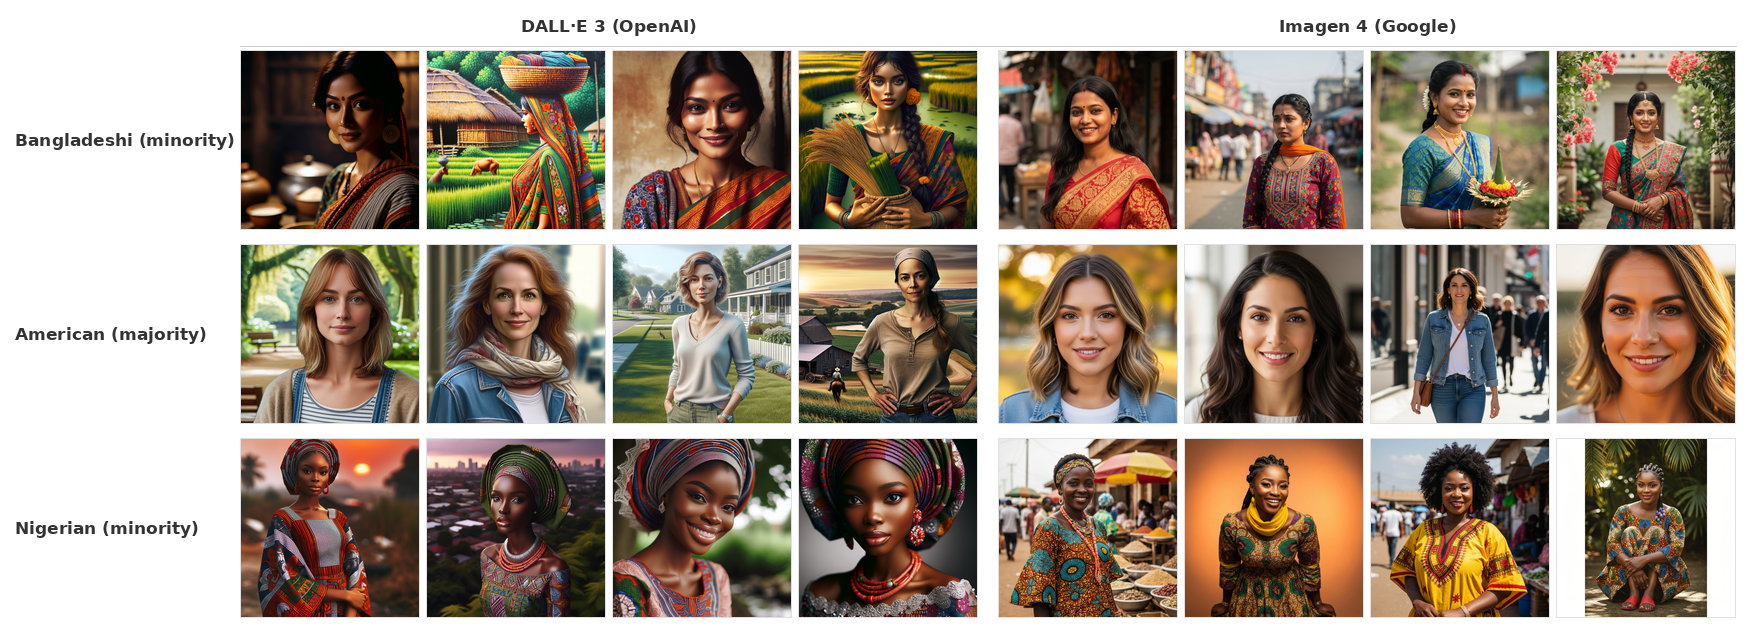
\includegraphics[width=\textwidth]{example_generations_grid.png}
 \caption{Example generations from DALL-E 3 and Imagen 4 for three cultural-identity prompts. Each row shows four independent generations for the same prompt. Within-prompt homogeneity is visually apparent, as is cross-model convergence: independently trained models produce aesthetically similar outputs for the same prompt.}
 \label{fig:grid}
\end{figure}

\subsection{Analysis 1: within-prompt diversity}

Across the 60 per-model prompt clusters (30 prompts $\times$ 2 models), the mean effective dimension was $d_{\mathrm{eff}} \approx 9.7$ out of 768 (10.4 for DALL-E 3, 9.1 for Imagen 4) - about 1.3\% of the available dimensions. Repeated generations from a single prompt occupy a roughly 10-dimensional subspace; the remaining dimensions carry negligible variance, consistent with outputs concentrated around a conditional mean. Averaged over both models, the three categories differed systematically (Figure~\ref{fig:a1}): open-ended prompts had the lowest effective dimension ($\bar{d}_{\mathrm{eff}} = 9.4$, against 9.9 for both other categories), artistic-style prompts the smallest support radius ($\bar{R}_\alpha = 0.425$), and cultural-identity prompts the largest values on both measures ($\bar{R}_\alpha = 0.548$ and $\bar{d}_{\mathrm{eff}} = 9.9$, against $\bar{R}_\alpha = 0.522$ for open-ended). The lowest effective dimension for open-ended prompts is consistent with the mechanism's prediction that the weakest conditioning permits the broadest averaging, though the ordering is not uniform across models: for Imagen 4 taken alone, cultural-identity prompts have the lowest $d_{\mathrm{eff}}$.

\begin{figure}[t]
 \centering
 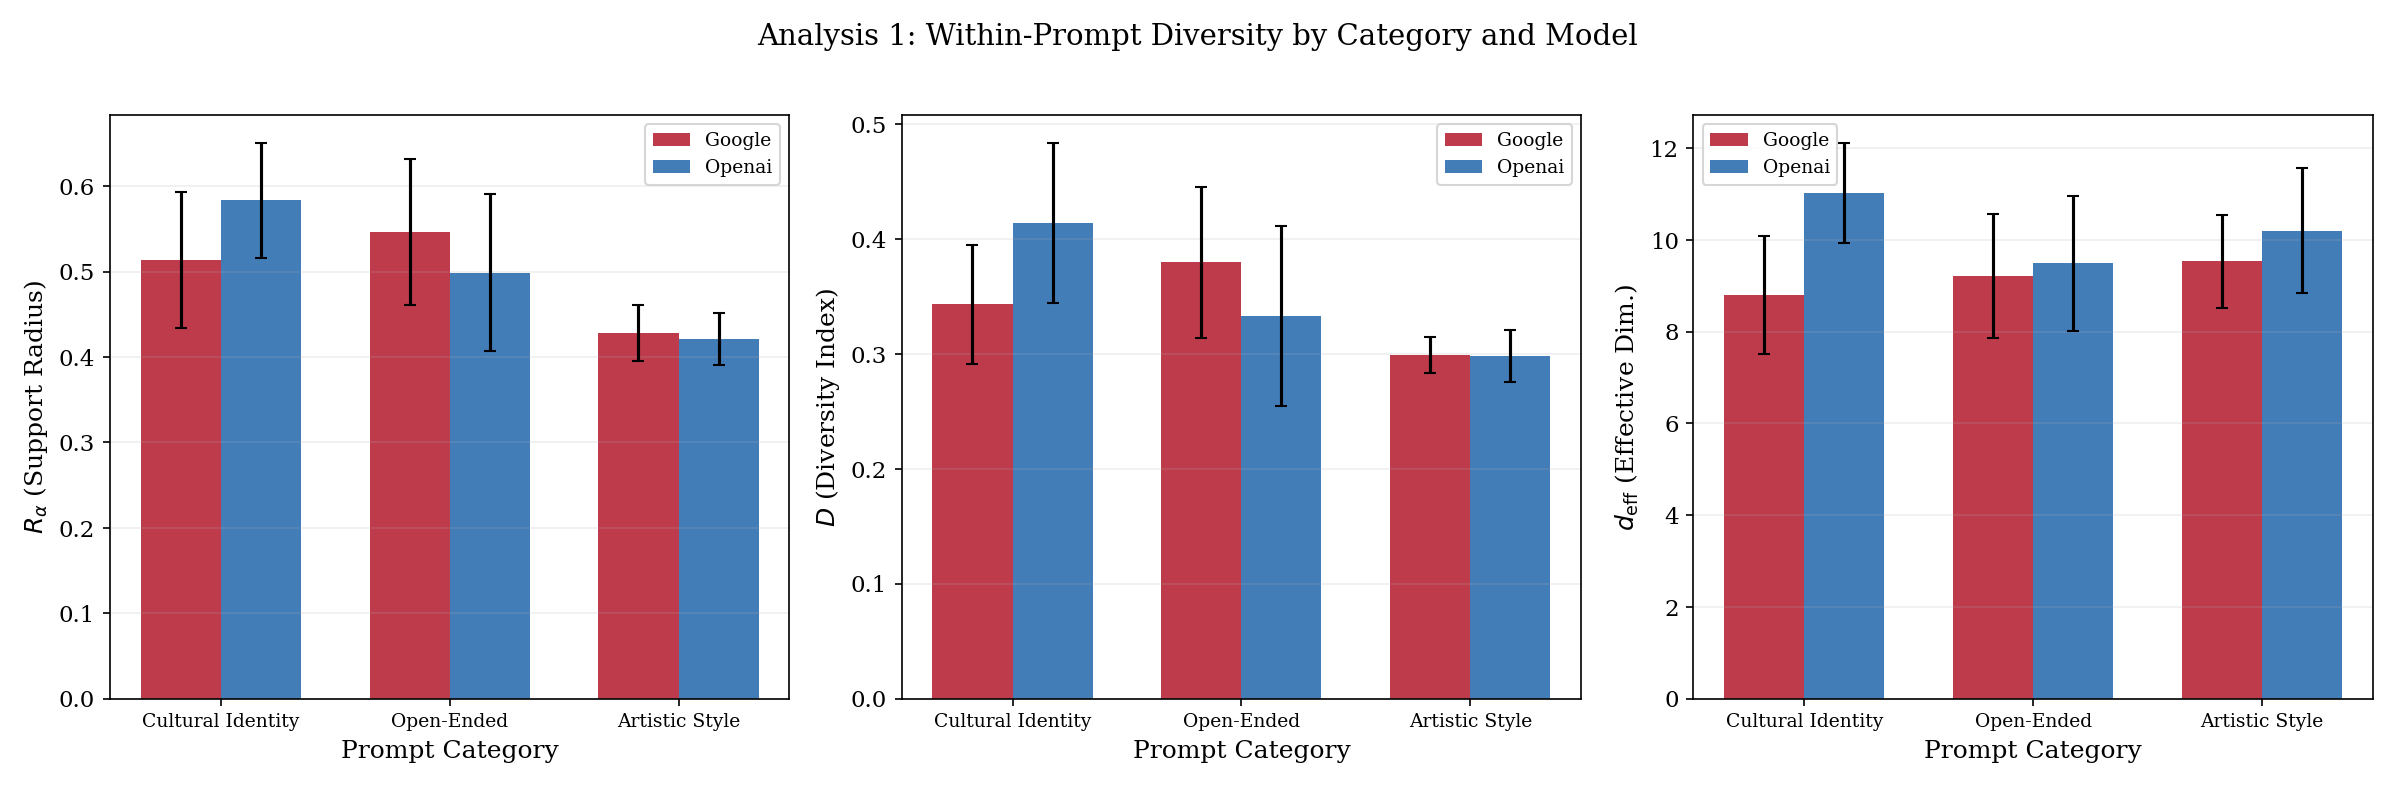
\includegraphics[width=\textwidth]{analysis1_within_prompt_diversity.png}
 \caption{Within-prompt diversity across the three prompt categories and both models, measured by effective support radius ($R_\alpha$), diversity index ($D$), and effective dimension ($d_{\mathrm{eff}}$). Open-ended prompts show the lowest effective dimension; artistic-style prompts the smallest support radius. Error bars show standard deviation across prompts within each category.}
 \label{fig:a1}
\end{figure}

\subsection{Analysis 2: minority mode suppression}

Pooling the per-model prompt clusters of both systems, majority nationalities exhibited a mean within-prompt support radius of $\bar{R}_\alpha = 0.618$, compared to $0.514$ for minority nationalities - a ratio of $0.83$, so minority representations are about 17\% less diverse (Figure~\ref{fig:a2}). A permutation test (10,000 permutations) and a 10,000-sample bootstrap confidence interval for the difference in means \citep{Efron1993, Good2000} confirm the gap ($p = 0.0002$; Hedges' $g = 1.51$). Because each nationality contributes one cluster per model, the pooled test treats correlated observations as independent; an exact cluster-aware permutation test at the nationality level ($n = 15$, averaging the two models within each nationality; all 3{,}003 label assignments enumerated) gives $p = 0.0007$, and the gap is significant within each model separately (DALL-E 3: exact $p = 0.0003$; Imagen 4: exact $p = 0.012$). The models do not merely underrepresent minority cultures in frequency; when they do appear, they are rendered with less internal variation, compressing each minority prompt into a tighter cluster. Pairwise cosine distances between nationality centroids are also strongly compressed (Figure~\ref{fig:heatmap}): rather than occupying well-separated regions, the different nationalities converge toward a shared aesthetic center.

\begin{figure}[t]
 \centering
 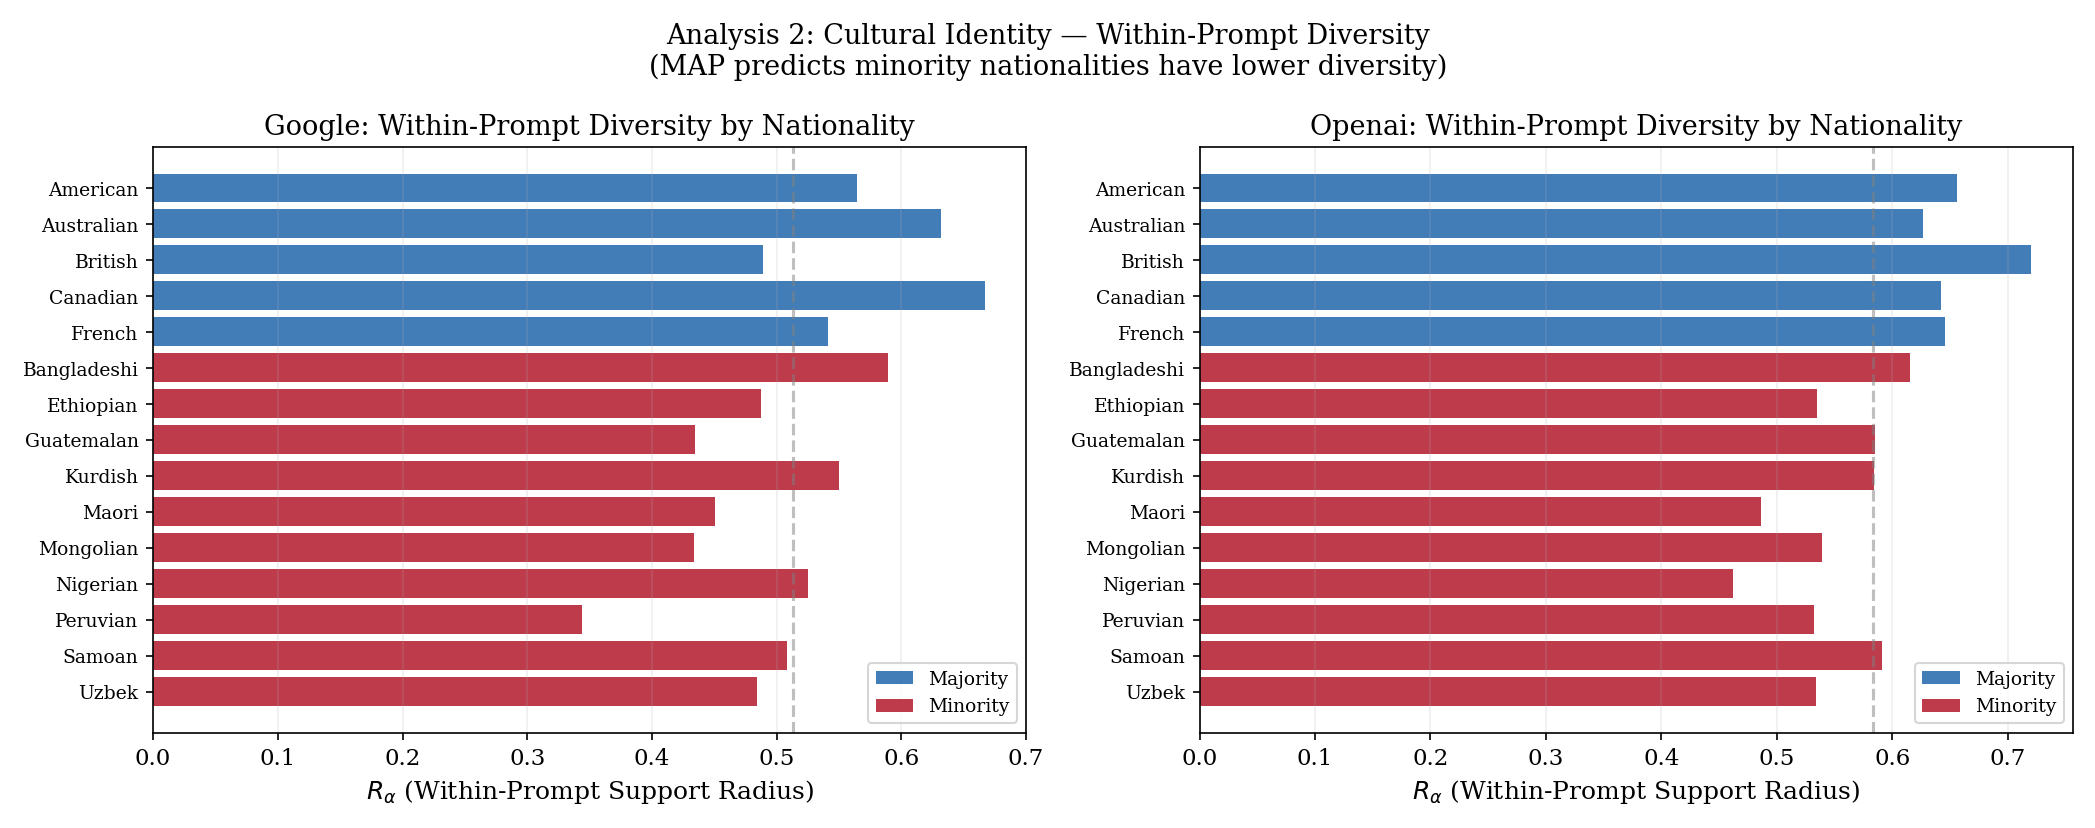
\includegraphics[width=\textwidth]{analysis2_cultural_convergence.png}
 \caption{Within-prompt diversity ($R_\alpha$) for cultural-identity prompts, grouped by majority and minority nationalities. Majority nationalities consistently show higher within-prompt diversity.}
 \label{fig:a2}
\end{figure}

\begin{figure}[t]
 \centering
 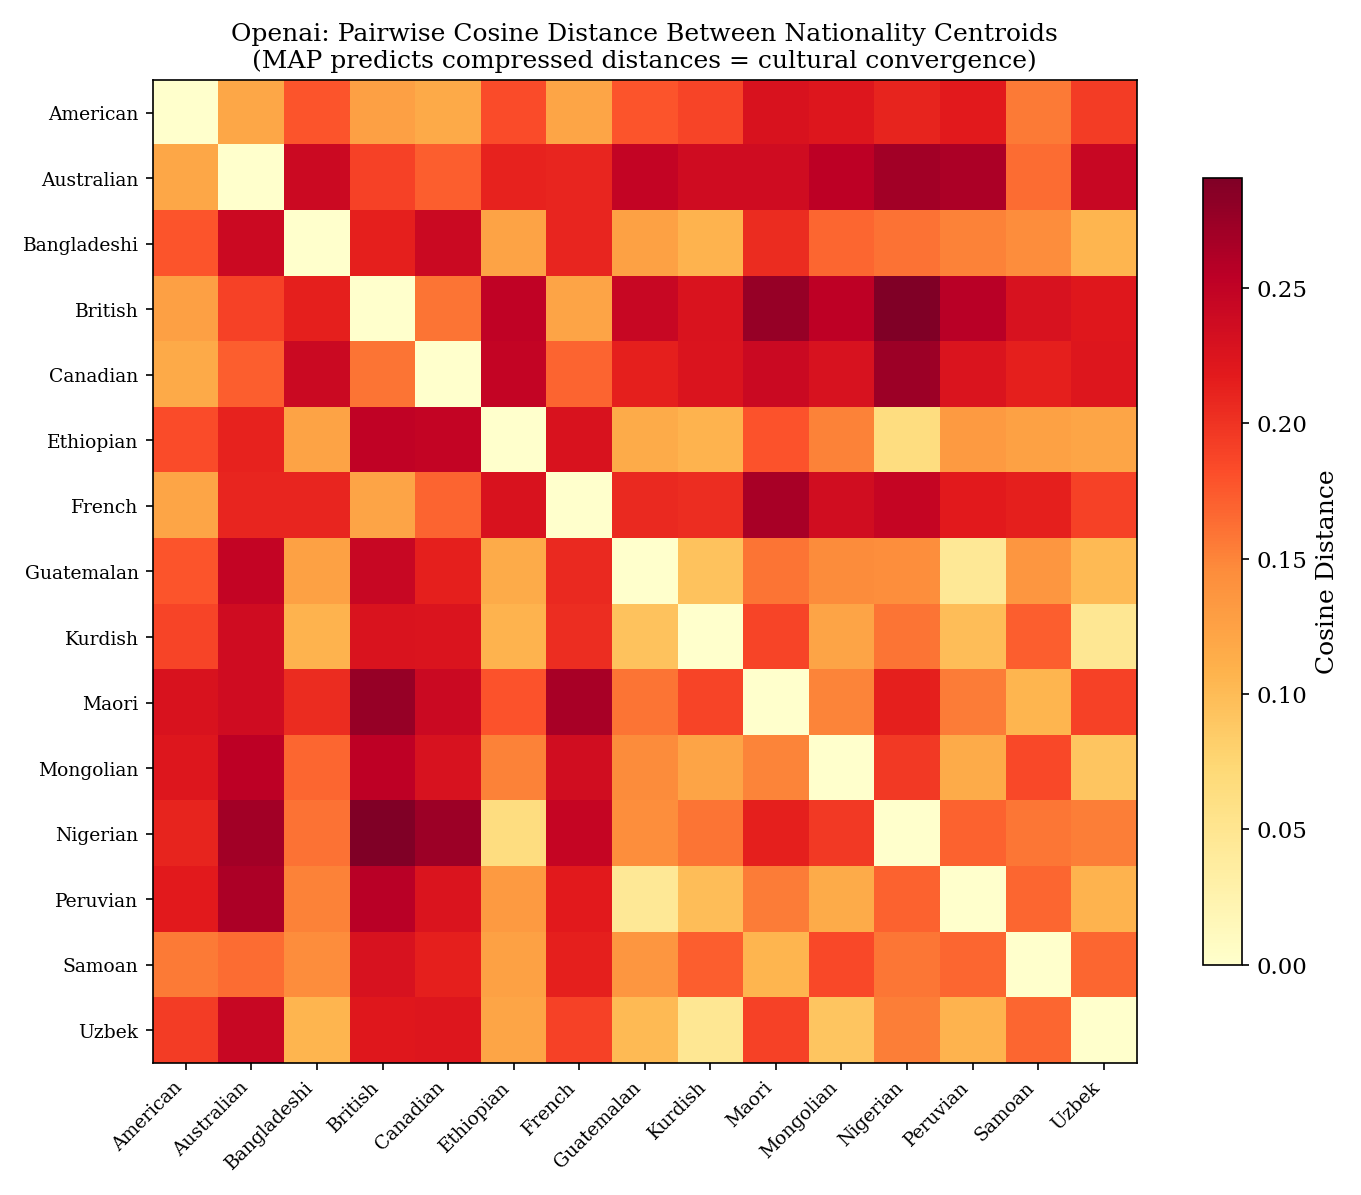
\includegraphics[width=0.85\textwidth]{analysis2_cultural_heatmap_openai.png}
 \caption{Pairwise cosine distance between nationality centroids in CLIP space (DALL-E 3). The compressed distances indicate convergence toward a shared aesthetic center across nationalities.}
 \label{fig:heatmap}
\end{figure}

\subsection{Analysis 3: cross-model convergence}

Across all 30 prompts, the mean cosine similarity between DALL-E 3 and Imagen 4 per-prompt centroids was $0.859$ (range $0.729$-$0.946$; Figure~\ref{fig:a3}). Isotropic random unit vectors in $\mathbb{R}^{768}$ would put this dozens of standard deviations above chance ($\mathrm{SD} \approx 1/\sqrt{768} \approx 0.036$), but that null is too weak: CLIP image embeddings occupy a narrow cone, so even \emph{mismatched} prompts produce substantial cross-model centroid similarity (mean $0.641$, SD $0.081$ over all $30 \times 29$ mismatched pairs). The matched-prompt mean exceeds this empirical baseline by $0.218$ - 2.7 standard deviations of the mismatched distribution - and the correspondence is nearly exact at the prompt level: for 27 of 30 prompts, the DALL-E 3 centroid's nearest neighbor among all 30 Imagen 4 centroids is its own matched prompt (chance expectation: 1). Two models from different companies, with different architectures and training data, occupy nearly the same region of semantic space for each prompt - not only in broad content but in pose, lighting, clothing, palette, and composition. This is the cross-model signature of a shared ``AI aesthetic'' that transcends any single system.

\begin{figure}[t]
 \centering
 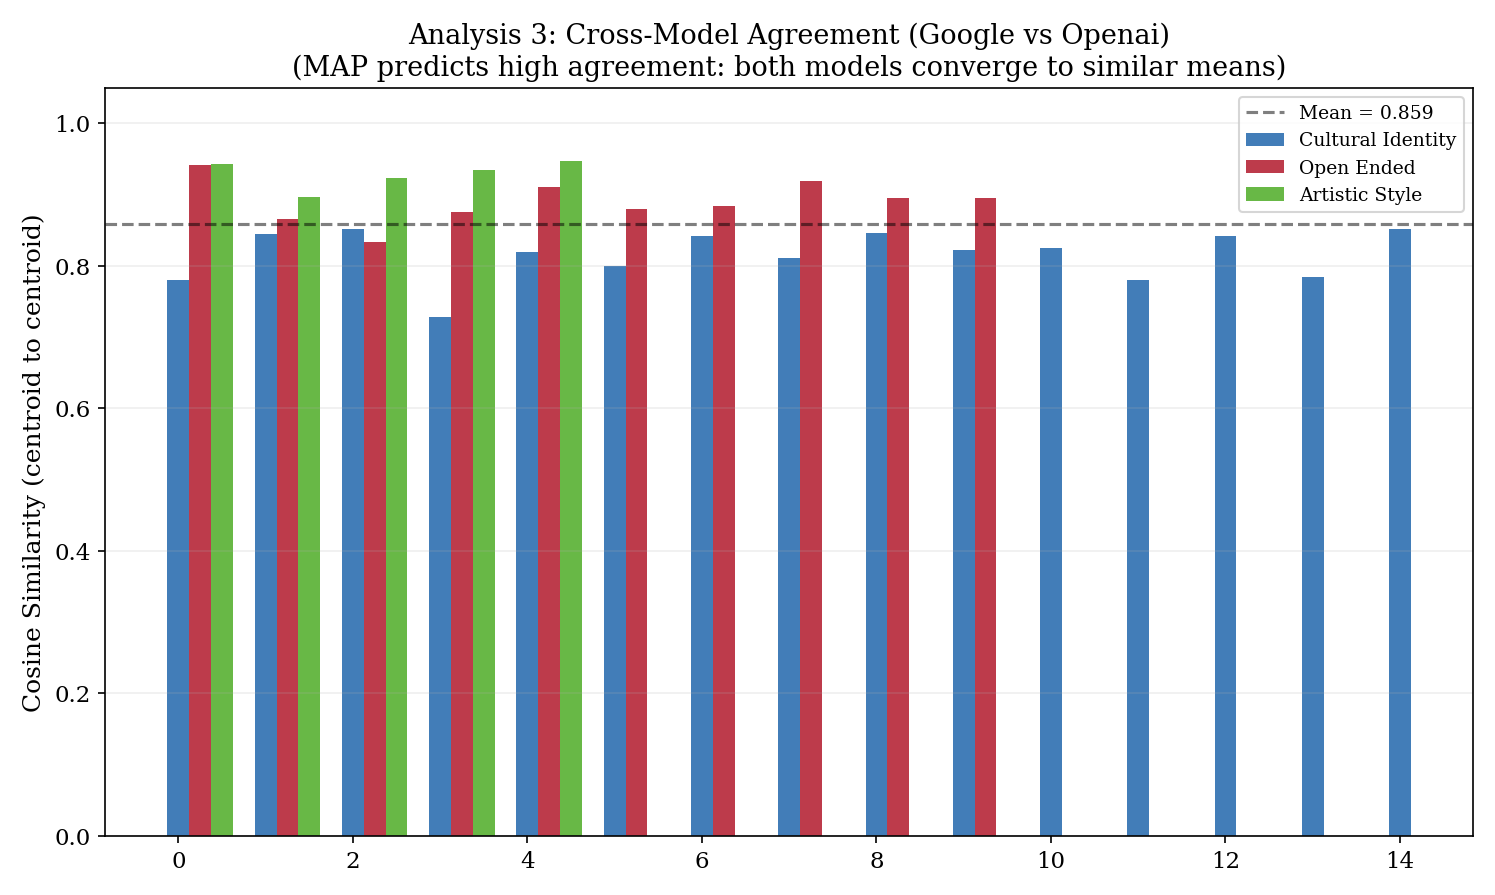
\includegraphics[width=\textwidth]{analysis3_cross_model_agreement.png}
 \caption{Cross-model agreement between DALL-E 3 and Imagen 4, measured as cosine similarity between per-prompt centroids across all 30 prompts. The mean matched-prompt similarity (0.859) substantially exceeds the mismatched-prompt baseline (0.641), indicating convergence to similar aesthetic centers.}
 \label{fig:a3}
\end{figure}

\subsection{Robustness}

Two checks confirm that these findings are not artifacts of the embedding model or of sampling noise. First, we re-embedded the images with DINOv2 - a self-supervised encoder trained on images alone, with no text-image alignment objective, producing 1,024-dimensional embeddings - and recomputed the measures (which are ratio-based or normalized per dimension, so they remain comparable across embedding spaces). The minority-suppression effect persists but is attenuated: on the cultural-identity prompts, the majority/minority $R_\alpha$ gap shrinks from 17.0\% under CLIP to 7.9\% under DINOv2, and the effective-dimension gap disappears. The per-prompt CLIP and DINOv2 $R_\alpha$ values correlate moderately (Pearson $r = 0.60$). CLIP thus appears to inflate the measured magnitude - plausibly because its text-image training imposes additional structure that compresses semantically similar concepts - but the pattern of stronger minority compression survives in a text-free embedding space, indicating it is a property of the images rather than of CLIP's alignment objective. We report the CLIP-based results as our primary analysis for comparability with prior work, while noting that the true magnitude likely lies between the two estimates. Second, per-prompt estimates are stable under resampling: 10,000-sample bootstrap confidence intervals for $R_\alpha$ have coefficients of variation typically below 10\% (median 5.6\%), so the differences between prompt categories and between majority and minority groups are well outside the range of sampling variability.

Table~\ref{tab:summary} summarizes the commercial-model results.

\begin{table}[t]
\centering
\caption{Summary of empirical measurements on commercial models.}
\label{tab:summary}
\begin{tabular}{@{}lll@{}}
\toprule
\textbf{Measurement} & \textbf{Statistic} & \textbf{Result} \\
\midrule
Within-prompt effective dimension & $d_{\mathrm{eff}} \approx 9.7 / 768$ & $\approx 1.3\%$ of dimensions \\
Open-ended $<$ constrained diversity & $\bar{d}_{\mathrm{eff}}$: 9.4 vs.\ 9.9 & As predicted \\
Minority $<$ majority diversity & $\bar{R}_\alpha$: 0.514 vs.\ 0.618 & 17\% gap ($p < 0.001$) \\
Cross-model convergence & $\cos = 0.859$ (30 prompts) & vs.\ 0.641 mismatched baseline \\
\bottomrule
\end{tabular}
\end{table}

\section{Ablation: objective versus preference training}\label{sec:ablation}

The commercial results are consistent with the MSE mechanism, but commercial models also undergo preference training (RLHF or DPO), content filtering, and curation, any of which could independently drive homogenization. To isolate the cause we use open-source models whose pipelines are transparent. We compare Stable Diffusion XL Base \citep{Podell2023}, trained only with the MSE objective on the LAION-5B dataset and given no preference training, against the same model fine-tuned with Direct Preference Optimization \citep{Rafailov2023}. The two share architecture, base data, and noise schedule; the only systematic difference is preference training, so any gap present in the base model cannot be attributed to it.

We varied model variant (Base vs.\ DPO) and classifier-free guidance scale ($w \in \{1.0, 5.0, 7.5, 15.0\}$) over 11 prompts (three majority and five minority cultural identities, three open-ended), generating 10 images per condition with fixed per-prompt seeds and the DPM++ 2M Karras scheduler at 30 steps - $2 \times 4 \times 11 \times 10 = 880$ images, embedded with the same CLIP pipeline.

\paragraph{Classifier-free guidance monotonically compresses diversity.} In the base model, mean $R_\alpha$ falls from $0.586$ at $w = 1.0$ to $0.407$ at $w = 15.0$ (a 30.5\% reduction) and $d_{\mathrm{eff}}$ from $7.06$ to $5.59$; the DPO model follows an identical monotonic trend ($R_\alpha$ $0.542 \to 0.403$; $d_{\mathrm{eff}}$ $6.63 \to 5.46$) at consistently lower diversity (Figure~\ref{fig:cfg}).

\begin{figure}[t]
 \centering
 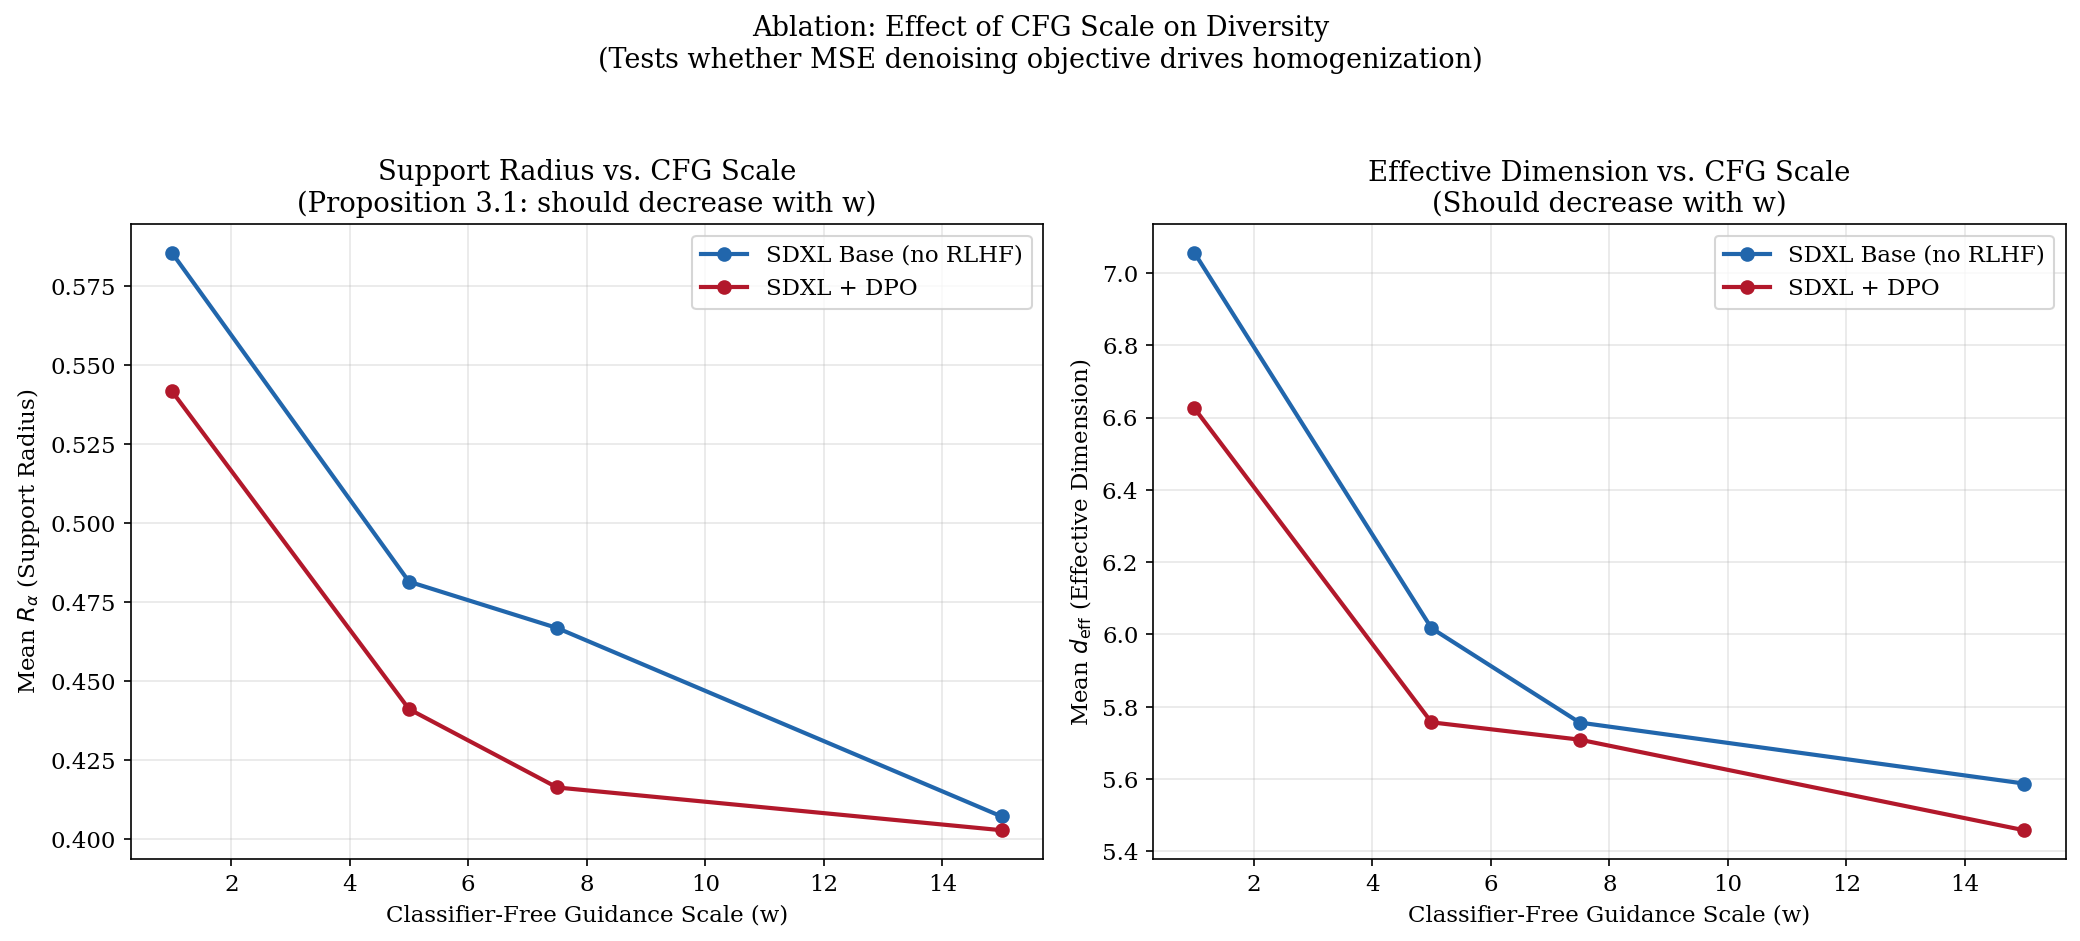
\includegraphics[width=\textwidth]{ablation_cfg_scale.png}
 \caption{Mean effective support radius and effective dimension versus classifier-free guidance scale for SDXL Base and SDXL + DPO. Both metrics decrease monotonically with guidance in both models; the DPO model is consistently lower.}
 \label{fig:cfg}
\end{figure}

\paragraph{The majority/minority gap exists without preference training.} This is the central result. At the standard guidance scale ($w = 7.5$), the base model - no preference training - shows a majority/minority diversity gap of 24.2\% (majority $\bar{R}_\alpha = 0.485$, minority $0.368$; gap $0.117$); the gap is present even at $w = 1.0$, where guidance adds no compression (12.4\%). Adding DPO at the same scale widens the gap modestly to 27.5\% (majority $0.469$, minority $0.340$; gap $0.129$). Approximately 91\% ($0.117/0.129$) of the gap observed in the preference-trained model is already present in the base model (Figure~\ref{fig:gap}); preference training contributes the remaining 9\%. Averaging across all four guidance scales gives the same conclusion (base 0.116 vs.\ DPO 0.122; 94\%).

\begin{figure}[t]
 \centering
 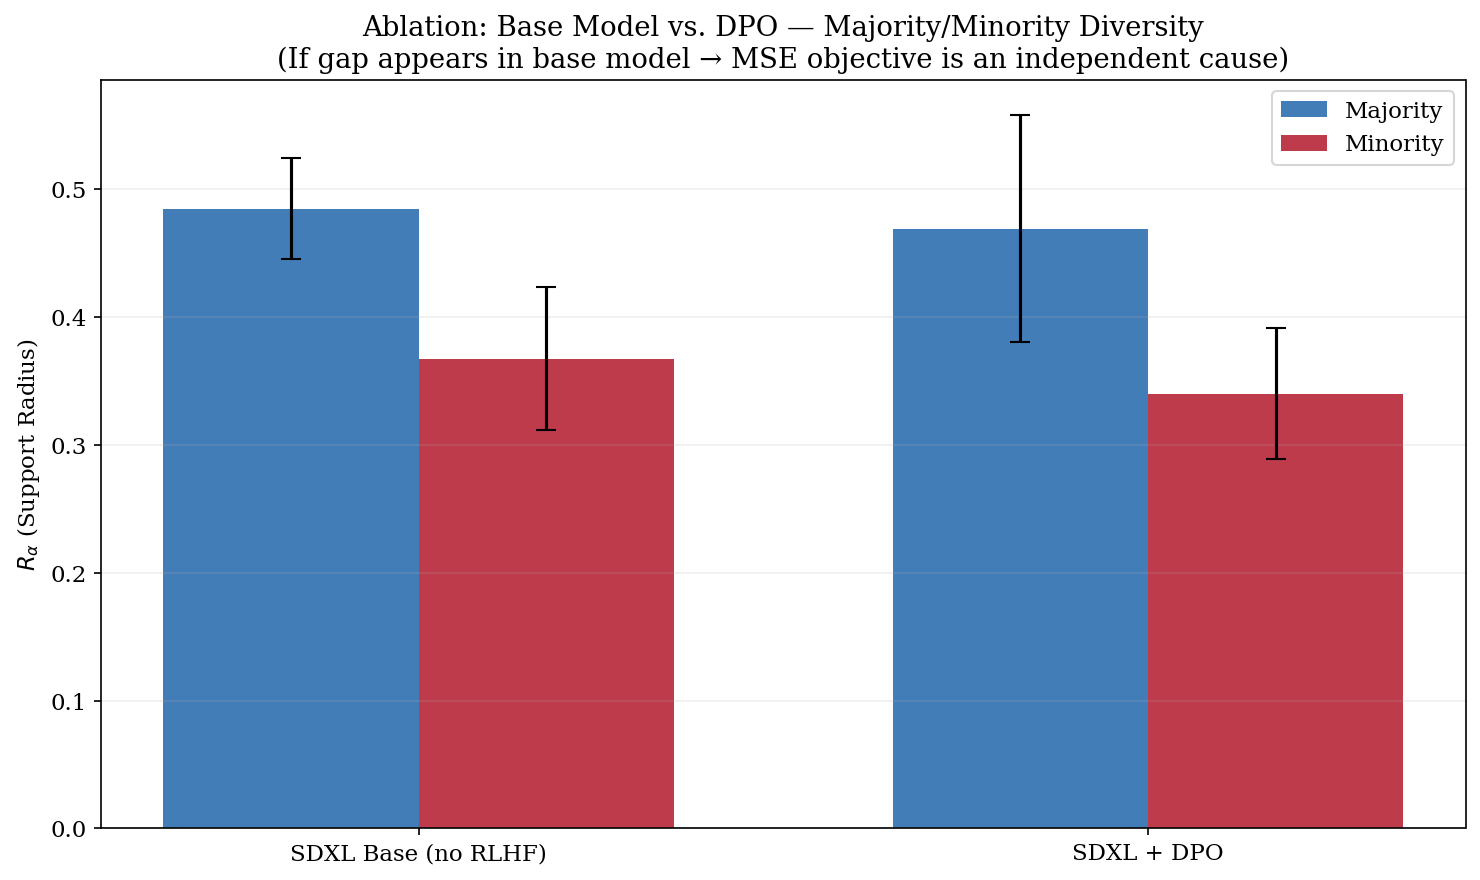
\includegraphics[width=\textwidth]{ablation_base_vs_dpo.png}
 \caption{Majority versus minority effective support radius for SDXL Base and SDXL + DPO at the standard guidance scale ($w = 7.5$). The gap is present in both; the base model exhibits 91\% of the gap seen in the preference-trained variant.}
 \label{fig:gap}
\end{figure}

Table~\ref{tab:ablation} decomposes the sources. The MSE objective is the primary structural contributor to the majority/minority gap; classifier-free guidance amplifies it substantially; preference training adds a further but comparatively modest contribution. Homogenization is therefore not primarily an artifact of RLHF or preference tuning - it is a structural property of the denoising objective, compounded by the standard mechanisms used to improve perceived quality.

\begin{table}[t]
\centering
\caption{Decomposition of homogenization sources (majority/minority $\bar{R}_\alpha$ gap).}
\label{tab:ablation}
\begin{tabular}{@{}llll@{}}
\toprule
\textbf{Configuration} & \textbf{Maj.\ $\bar{R}_\alpha$} & \textbf{Min.\ $\bar{R}_\alpha$} & \textbf{Gap} \\
\midrule
SDXL Base, $w = 1.0$ (no CFG, no pref.) & 0.656 & 0.575 & 12.4\% \\
SDXL Base, $w = 7.5$ (CFG, no pref.) & 0.485 & 0.368 & 24.2\% \\
SDXL + DPO, $w = 7.5$ (CFG + pref.) & 0.469 & 0.340 & 27.5\% \\
\bottomrule
\end{tabular}
\end{table}

\section{Discussion}

The measurements give quantitative content to a claim that has largely been made qualitatively. Commercial text-to-image models discard the overwhelming majority of aesthetic variation for any given prompt, compress minority cultural representations more than majority ones, and converge - across companies - on a shared visual center. The ablation locates the primary cause in the training objective itself rather than in downstream human-feedback tuning, which reframes homogenization from a data-and-alignment problem into a problem of objective design. Interventions aimed only at curating training data or adjusting preference models therefore address a secondary contributor; the dominant effect is upstream, in what an expectation-minimizing objective does to low-mass modes.

The methodology is deliberately model-agnostic and cheap to run: it requires only prompt-conditioned samples, an embedding model, and the three measures, and it applies to any generative image model exposed through an API or open weights. This makes it suitable for auditing and for longitudinal monitoring - for example, tracking whether successive model releases become more or less homogenizing, or whether a ``sovereign'' model trained in a specific cultural context escapes the global mean or inherits it.

For communication research, the result reframes a familiar concern. Generative models are increasingly used to produce the images that circulate on platforms, in advertising, and in news and civic contexts, and are often treated as neutral or representative depictions. Our measurements show that, for any given prompt, these systems return a narrow band of the possible visual space, and that the band is narrower still for less-represented cultures. Measuring this concentration - rather than only inspecting individual outputs - gives the field a quantitative handle on representational narrowing that can be compared across systems, tracked over time, and related to downstream questions about what audiences see. The approach sits naturally alongside computational work on visual culture and platform analysis, where embedding-based measures are already used to study large image collections.

The finding also has a concrete design implication. Because the dominant contributor is the training objective rather than preference tuning, interventions that operate only on data curation or reward modeling address a secondary term. Measurably reducing homogenization is likely to require changes to the generative objective itself - for example, objectives that explicitly reward within-prompt diversity or penalize collapse toward the conditional mean. Whatever the intervention, the measures proposed here supply an evaluation target: a diversity-preserving model should raise within-prompt effective dimension and narrow the majority/minority gap without sacrificing prompt fidelity.

\paragraph{Limitations.} Diversity here is measured in embedding space, so results are relative to the encoder; we mitigate this by replicating with DINOv2, but no embedding is neutral. Our prompts operationalize ``majority'' and ``minority'' through nationality and artistic style, a deliberate simplification of culture. The design is also modest in scale - roughly 20 images per prompt and 15 nationalities - so the headline percentages carry the sampling uncertainty quantified by the bootstrap and exact permutation analyses above, and should be read as estimates of direction and rough magnitude rather than precise population parameters. Commercial APIs are moving targets, and generation involved occasional filtering and errors that slightly reduced per-prompt counts. Finally, effective dimension and support radius capture concentration, not the normative question of which concentrations are harmful; that interpretation is developed in the companion paper.

\section{Conclusion}

We have introduced and applied a reproducible methodology for measuring aesthetic and cultural diversity collapse in text-to-image models. Across 1,177 commercial images and an 880-image open-source ablation, the outputs are highly concentrated, more so for minority cultures, and convergent across independently developed systems - and the ablation attributes the effect primarily to the MSE denoising objective. The measurements are consistent with, and were guided by, the mathematical framework of Section~\ref{sec:mechanism}; their broader cultural and critical interpretation is developed in a companion paper \citep{Companion2026}. We release all prompts, code, and embeddings to support replication and extension to other models and cultural contexts.

\section*{Data and code availability}
All prompts, generation and analysis code, and precomputed CLIP and DINOv2 embeddings are available at the project repository (archived on Zenodo). % For anonymized review, this link is removed; the repository is public on publication.
The raw generated images are not redistributed (owing to provider terms, size, and the sensitivity of AI-generated images of people) but can be regenerated from the released prompts and generation scripts.

\section*{Declarations}
\textbf{Funding.} Supported by the Australian Research Council Centre of Excellence for Automated Decision-Making and Society (CE200100005). \textbf{Competing interests.} The authors declare no competing interests. \textbf{Use of AI tools.} Commercial and open-source generative models (DALL-E 3, Imagen 4, Stable Diffusion XL) were used to produce the image corpora analyzed as data; no generative AI tool was used for the conceptualization, analysis, or autonomous authoring of the manuscript. \textbf{Author contributions.} All authors contributed to the conception, design, and methodology of the study. The mathematical framework was developed by T.\ Graham, V.\ Padinjaredath Suresh, A.\ Snoswell, D.\ Angus, K.\ Witzenberger, W.\ He, G.\ Zhu, A.\ Obeid, and K.\ Chand; the empirical experiments and analysis were conducted by T.\ Graham. All authors read and approved the final manuscript. \textbf{Companion paper.} A companion paper develops the cultural and critical interpretation of these findings; both are being made available as preprints and disclosed to the editors.

\bibliography{refs}

\end{document}
